\documentclass{article}

% 33.1 inches by 46.8 inches
% 841 mm by 1189 mm
\usepackage[a0paper, landscape, margin=.3in, top=1in]{geometry}

% Grid size of 1.48 inches
% Need: 16x31 grid.
% 23 in by 45.88 in

% margin of .3 inches keeps us within bounds.

\usepackage{tikz}

\setlength{\parindent}{0pt}

\begin{document}
\begin{center}
\scalebox{8}{Rule 90}\\[1in]
\begin{tikzpicture}[scale=3.3]
  \def\i{0}
  \draw[fill=black] (\i + 0, 0) rectangle (\i + 1, 1);
  \draw[fill=black] (\i + 1, 0) rectangle (\i + 2, 1);
  \draw[fill=black] (\i + 2, 0) rectangle (\i + 3, 1);
  \draw[fill=gray] (\i + 1,-1) rectangle (\i + 2, 0);

  \def\i{4}
  \draw[fill=black] (\i + 0, 0) rectangle (\i + 1, 1);
  \draw[fill=black] (\i + 1, 0) rectangle (\i + 2, 1);
  \draw[fill=gray] (\i + 2, 0) rectangle (\i + 3, 1);
  \draw[fill=black] (\i + 1,-1) rectangle (\i + 2, 0);

  \def\i{8}
  \draw[fill=black] (\i + 0, 0) rectangle (\i + 1, 1);
  \draw[fill=gray] (\i + 1, 0) rectangle (\i + 2, 1);
  \draw[fill=black] (\i + 2, 0) rectangle (\i + 3, 1);
  \draw[fill=gray] (\i + 1,-1) rectangle (\i + 2, 0);

  \def\i{12}
  \draw[fill=black] (\i + 0, 0) rectangle (\i + 1, 1);
  \draw[fill=gray] (\i + 1, 0) rectangle (\i + 2, 1);
  \draw[fill=gray] (\i + 2, 0) rectangle (\i + 3, 1);
  \draw[fill=black] (\i + 1,-1) rectangle (\i + 2, 0);

  \def\i{16}
  \draw[fill=gray] (\i + 0, 0) rectangle (\i + 1, 1);
  \draw[fill=black] (\i + 1, 0) rectangle (\i + 2, 1);
  \draw[fill=black] (\i + 2, 0) rectangle (\i + 3, 1);
  \draw[fill=black] (\i + 1,-1) rectangle (\i + 2, 0);

  \def\i{20}
  \draw[fill=gray] (\i + 0, 0) rectangle (\i + 1, 1);
  \draw[fill=black] (\i + 1, 0) rectangle (\i + 2, 1);
  \draw[fill=gray] (\i + 2, 0) rectangle (\i + 3, 1);
  \draw[fill=gray] (\i + 1,-1) rectangle (\i + 2, 0);

  \def\i{24}
  \draw[fill=gray] (\i + 0, 0) rectangle (\i + 1, 1);
  \draw[fill=gray] (\i + 1, 0) rectangle (\i + 2, 1);
  \draw[fill=black] (\i + 2, 0) rectangle (\i + 3, 1);
  \draw[fill=black] (\i + 1,-1) rectangle (\i + 2, 0);

  \def\i{28}
  \draw[fill=gray] (\i + 0, 0) rectangle (\i + 1, 1);
  \draw[fill=gray] (\i + 1, 0) rectangle (\i + 2, 1);
  \draw[fill=gray] (\i + 2, 0) rectangle (\i + 3, 1);
  \draw[fill=gray] (\i + 1,-1) rectangle (\i + 2, 0);
\end{tikzpicture}

\vspace{2in}
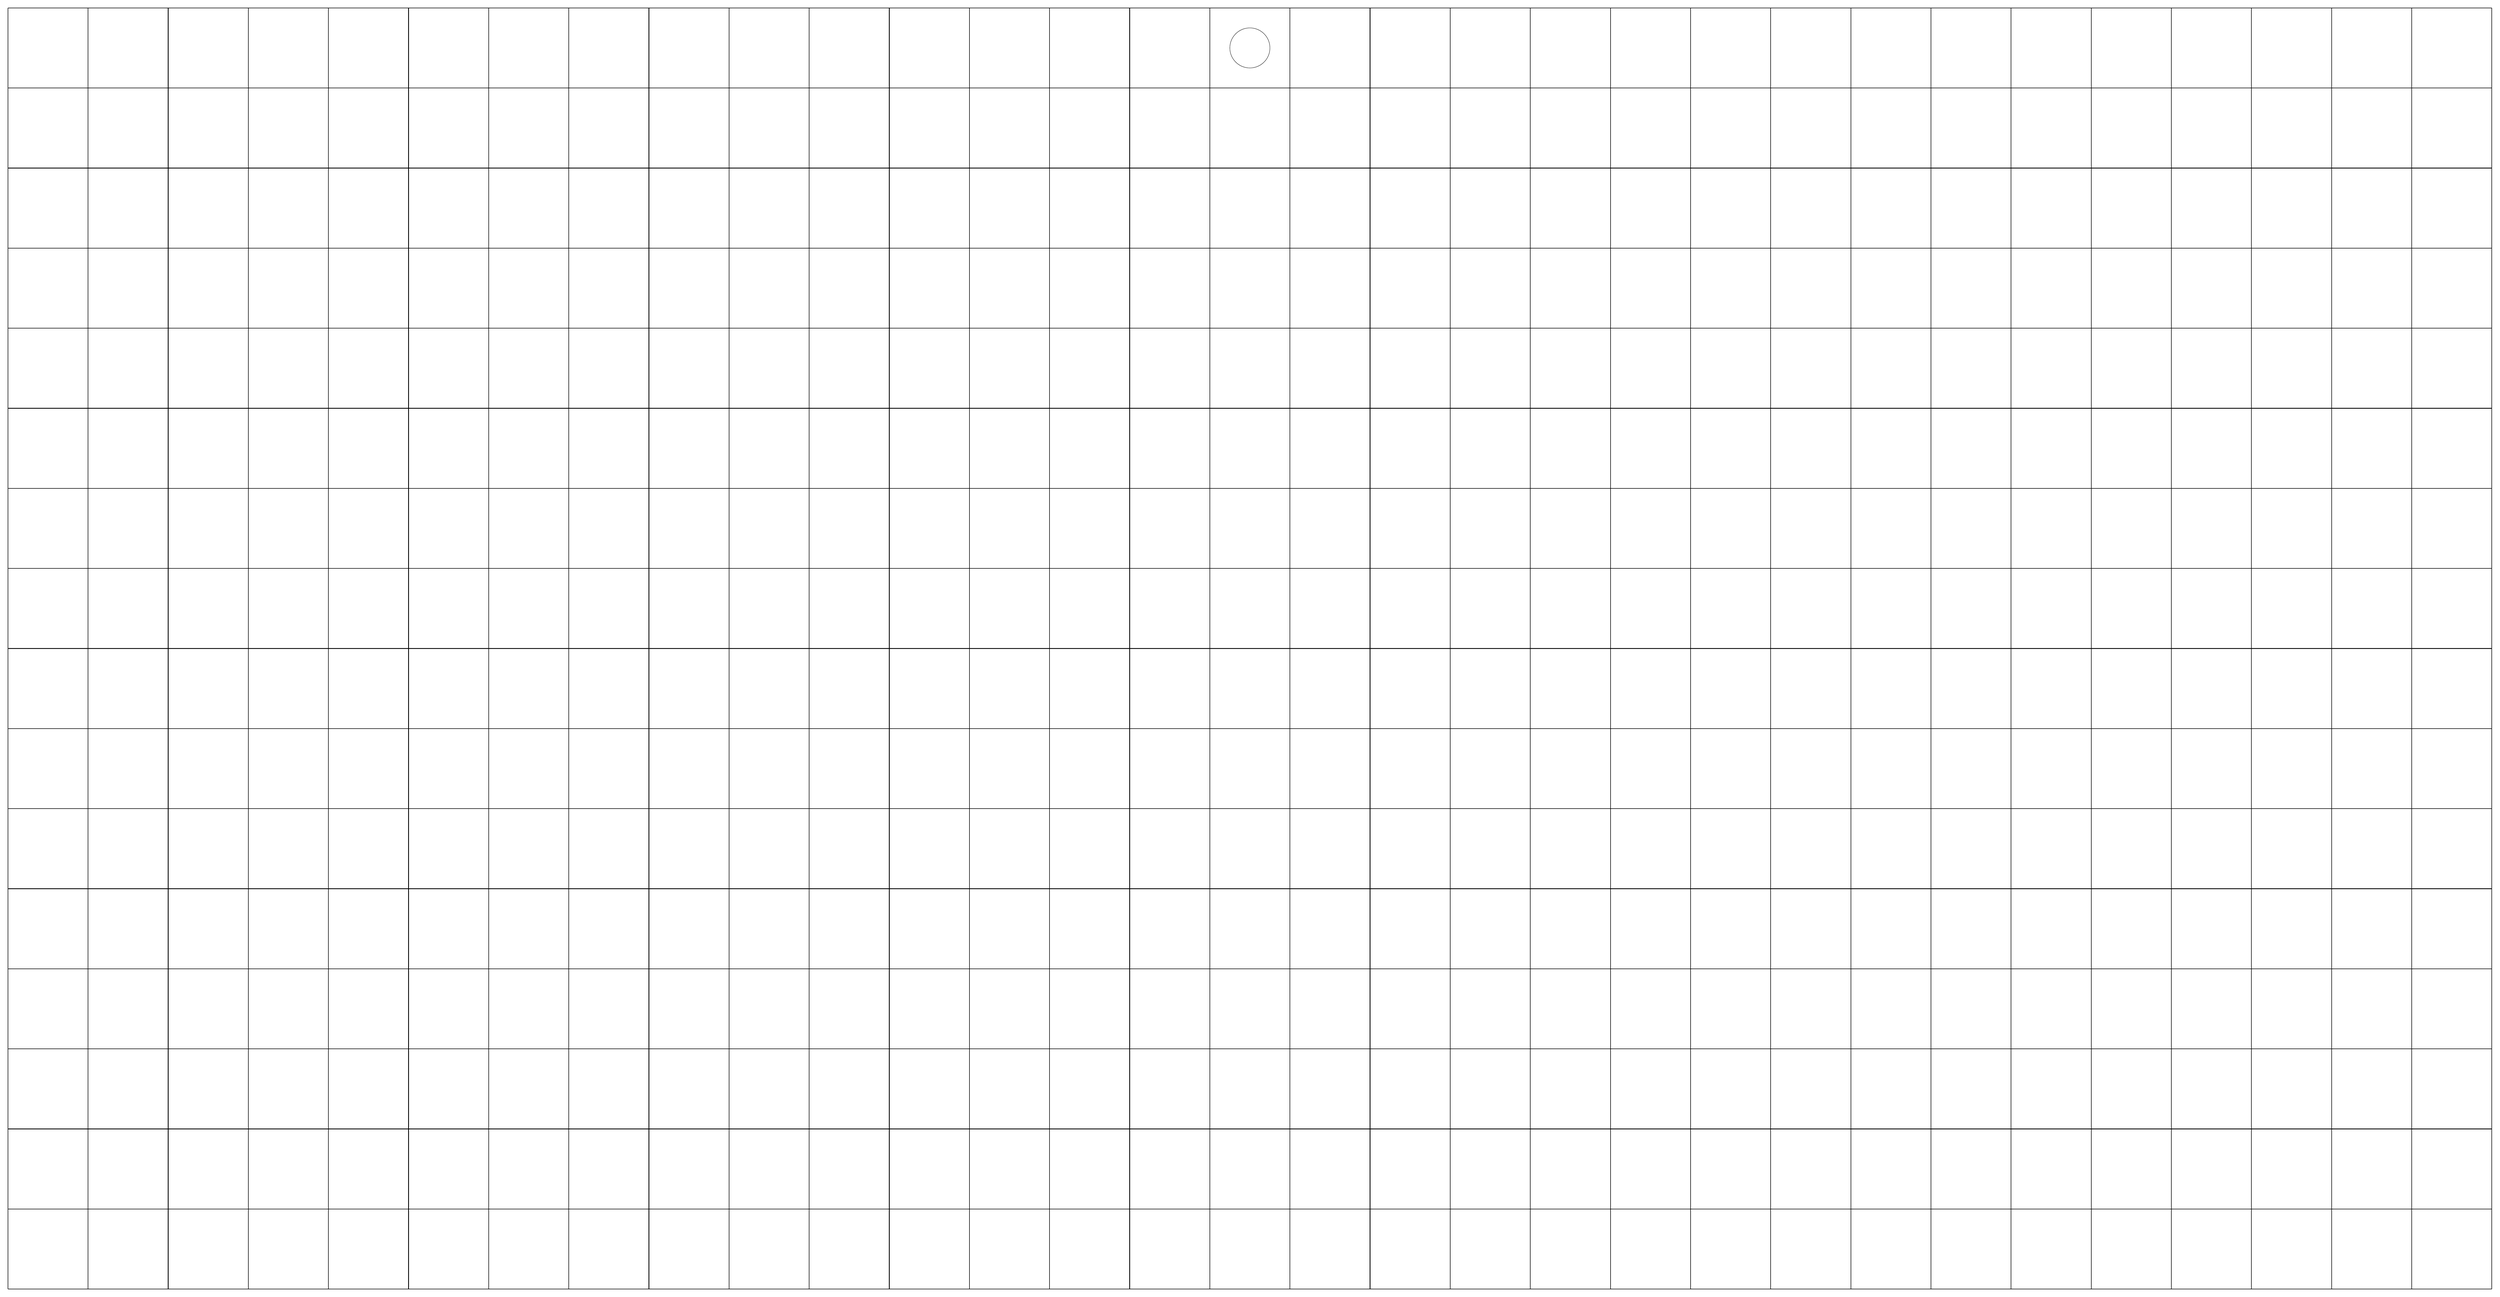
\begin{tikzpicture}[scale=3.7]
\draw[step=1, black, thick] (0,0) grid (31,16);
\draw (15.5, 15.5) circle (.25);
\end{tikzpicture}
\end{center}

\end{document}

